\documentclass[12pt]{article}

 %%%
 \usepackage[utf8]{inputenc}
 \usepackage{graphicx}
 \usepackage{xcolor}
 \usepackage{hyperref}
 \hypersetup{colorlinks, linkcolor = black, citecolor = black, filecolor = black, urlcolor = [RGB]{227, 114, 34}}
 \usepackage{float}
 \usepackage{geometry}\geometry{a4paper, total={170mm,257mm}, left=20mm, top=20mm}

 \definecolor{PIKorange}{RGB}{227, 114, 34}
 \definecolor{PIKgray}{RGB}{142, 144, 143}

 \title{ \bfseries \color{PIKorange} Eq. Guinea: information on national emissions, population and GDP, and mitigation targets}

 %%%

 \begin{document}

 \maketitle

 %%%
 \noindent \textbf{Authors:} \newline
 \indent Annika Guenther$^{1}$ \newline
 \indent Johannes Guetschow$^{1}$ \newline
 \noindent \textbf{Affiliations:} \newline
 \indent 1. Potsdam Institute for Climate Impact Research, Germany \newline
 \noindent \textbf{DOI:} [to be added] \newline

 \textbf{TODO}
 \begin{itemize}
 \item Table with info on target (main and reclass; emissions from NDC; target quantis + plot).
 \item GWP: NDC emissions coverted from AR2 to AR4 by national conversion factor (2010--2017, PRIMAP-hist v2.1).
 \item References!
 \end{itemize}

 \newpage %%%
 \section{Emissions and socio-economic data}
 \label{sec:nonLULUCFSocioEco}
 With national emissions of 13.0~Mt CO$_2$eq, Eq. Guinea contributed 0.02\% to global emissions in 2017, and in 2030 its share is estimated to stay at a similar level (Table~\ref{tab:overview}).
 The estimates for 2030 are based on the downscaled SSP2 Middle of the Road marker scenario (dmSSP2), in which Eq. Guinea is estimated to emit 16.6~Mt CO$_2$eq in 2030.
 That change in emissions would constitute a substantial increase of 27.4\% compared to 2017. 
 The pathways dmSSP1--5 show a range of 14.1--18.9~Mt CO$_2$eq in 2030, and 11.1--24.9~Mt CO$_2$eq in 2050.
 The country's global rank in terms of total emissions per unit of GDP was 59 in 2017, and 37 regarding the per-capita emissions (55 and 39 in 2030).
 In terms of accumulated historical emissions, Eq. Guinea contributed to the global 1850--2017 emissions by 0.01\%. 
 When only accounting for the years 1990--2017, its contribution increases to 0.02\%.
 All of the emissions are presented following GWP~AR4, and exclude emissions from LULUCF (exclLU), and bunkers fuels emissions (exclBunkers).

 \begin{table}[H]
 \centering
 \caption{National emissions (dmSSP2), GDP and population for Eq. Guinea, together with the emissions per unit of GDP and per capita emissions (all for 2017 and 2030). 
 Additionally, the global share and its rank are displayed.}
 \label{tab:overview}
 \begin{tabular}{l || l r l r r}
 \bfseries  & \bfseries Year & \bfseries Total & \bfseries Unit & \bfseries Glob. share & \bfseries Rank \tabularnewline \hline \hline
 \bfseries Emissions & 2017 & 13.0 & Mt CO$_2$eq & 0.02\% & 136 \tabularnewline 
 \bfseries  & 2030 & 16.6 & Mt CO$_2$eq & 0.02\% & 132 \tabularnewline \hline
 \bfseries GDP & 2017 & 20.2 & Billion 2011~GK\$ & 0.01\% & 144 \tabularnewline 
 \bfseries  & 2030 & 38.3 & Billion 2011~GK\$ & 0.02\% & 143 \tabularnewline \hline
 \bfseries Emissions & 2017 & 0.6 & t CO$_2$eq / Thousand 2011~GK\$ & 0.6\% & 59 \tabularnewline 
 \bfseries per GDP & 2030 & 0.4 & t CO$_2$eq / Thousand 2011~GK\$ & 0.6\% & 55 \tabularnewline \hline
 \bfseries Population & 2017 & 1.3 & Million Pers & 0.01\% & 154 \tabularnewline 
 \bfseries  & 2030 & 1.6 & Million Pers & 0.01\% & 151 \tabularnewline \hline
 \bfseries Emissions & 2017 & 10.3 & t CO$_2$eq /  Pers & 0.7\% & 37 \tabularnewline 
 \bfseries per capita & 2030 & 10.1 & t CO$_2$eq /  Pers & 0.7\% & 39 \tabularnewline 
 \end{tabular}
 \end{table}

 For Eq. Guinea, in 2017 the main emissions share on sectoral level (Fig.~\ref{fig:tsEmi}) came from the Energy sector (87.8\%), followed by IPPU (9.3\%)
 The Kyoto~GHG with the highest emissions in 2017 was CO$_2$, constituting  55.4\% of the national emissions. 
 Second largest contributor was CH$_4$ (44.3\%)
 The total of F-gasesonly represented 0.0\%.
 The trend in total emissions is mostly driven by CH$_4$ emissions from the Energy sector, which contributed 40.9\% to Eq. Guinea's 2017 emissions.\footnote{Analysis based on the correlations between total national emissions (exclLU) versus the emissions of the combinations of main-sectors \& the gases CO$_2$, CH$_4$, N$_2$O and F-gases. 
 Only data from 2010 to 2017 are assessed. 
 The (up to) three gas \& sector combinations are chosen for which the slope of the regression line to the correlated values exceeds 0.2.}
 The total CO$_2$ emissions are expected to be 59.7\% of the national Kyoto~GHG emissions in 2030 (dmSSP2).

 \begin{figure}[H]
 \centering
 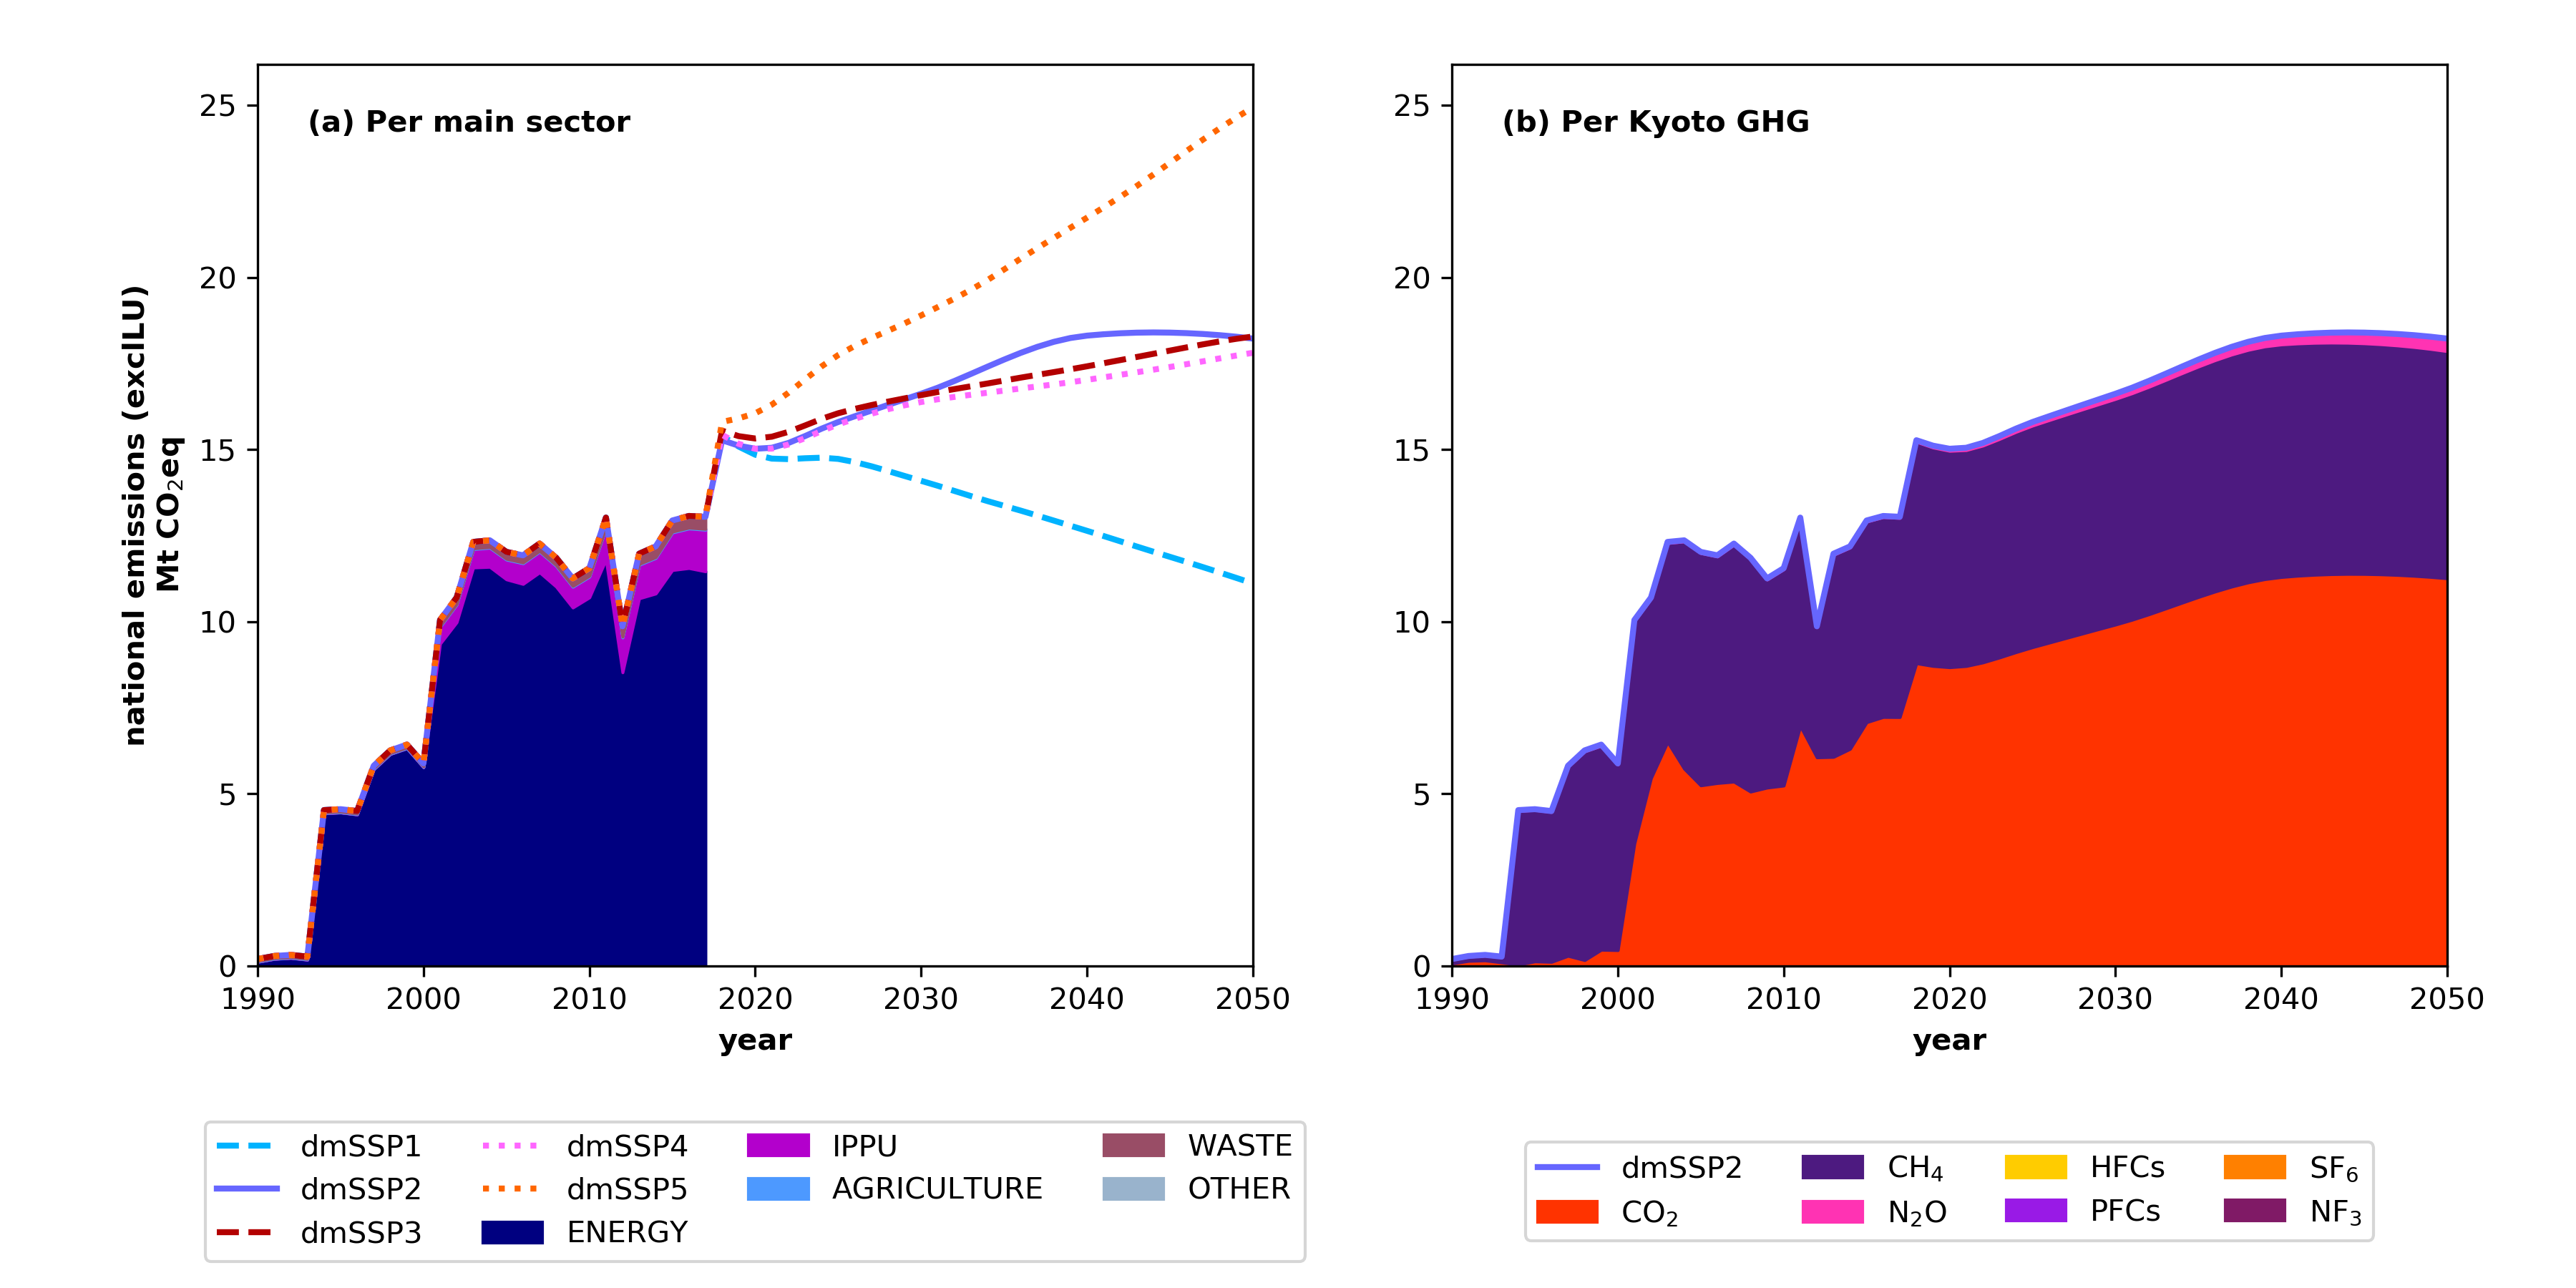
\includegraphics[width=\textwidth]{C:/Users/annikag/primap/ndc_quantifications/latex_files/GNQ/ts_emi_exclLU_GNQ.png}
 \caption{'Stacked' timeseries of national emissions (exclLU) per main-sector (a) and Kyoto~GHG (b). 
 No information available on the sectoral contributions after 2017.}
 \label{fig:tsEmi}
 \end{figure}

 \begin{figure}[H]
 \centering
 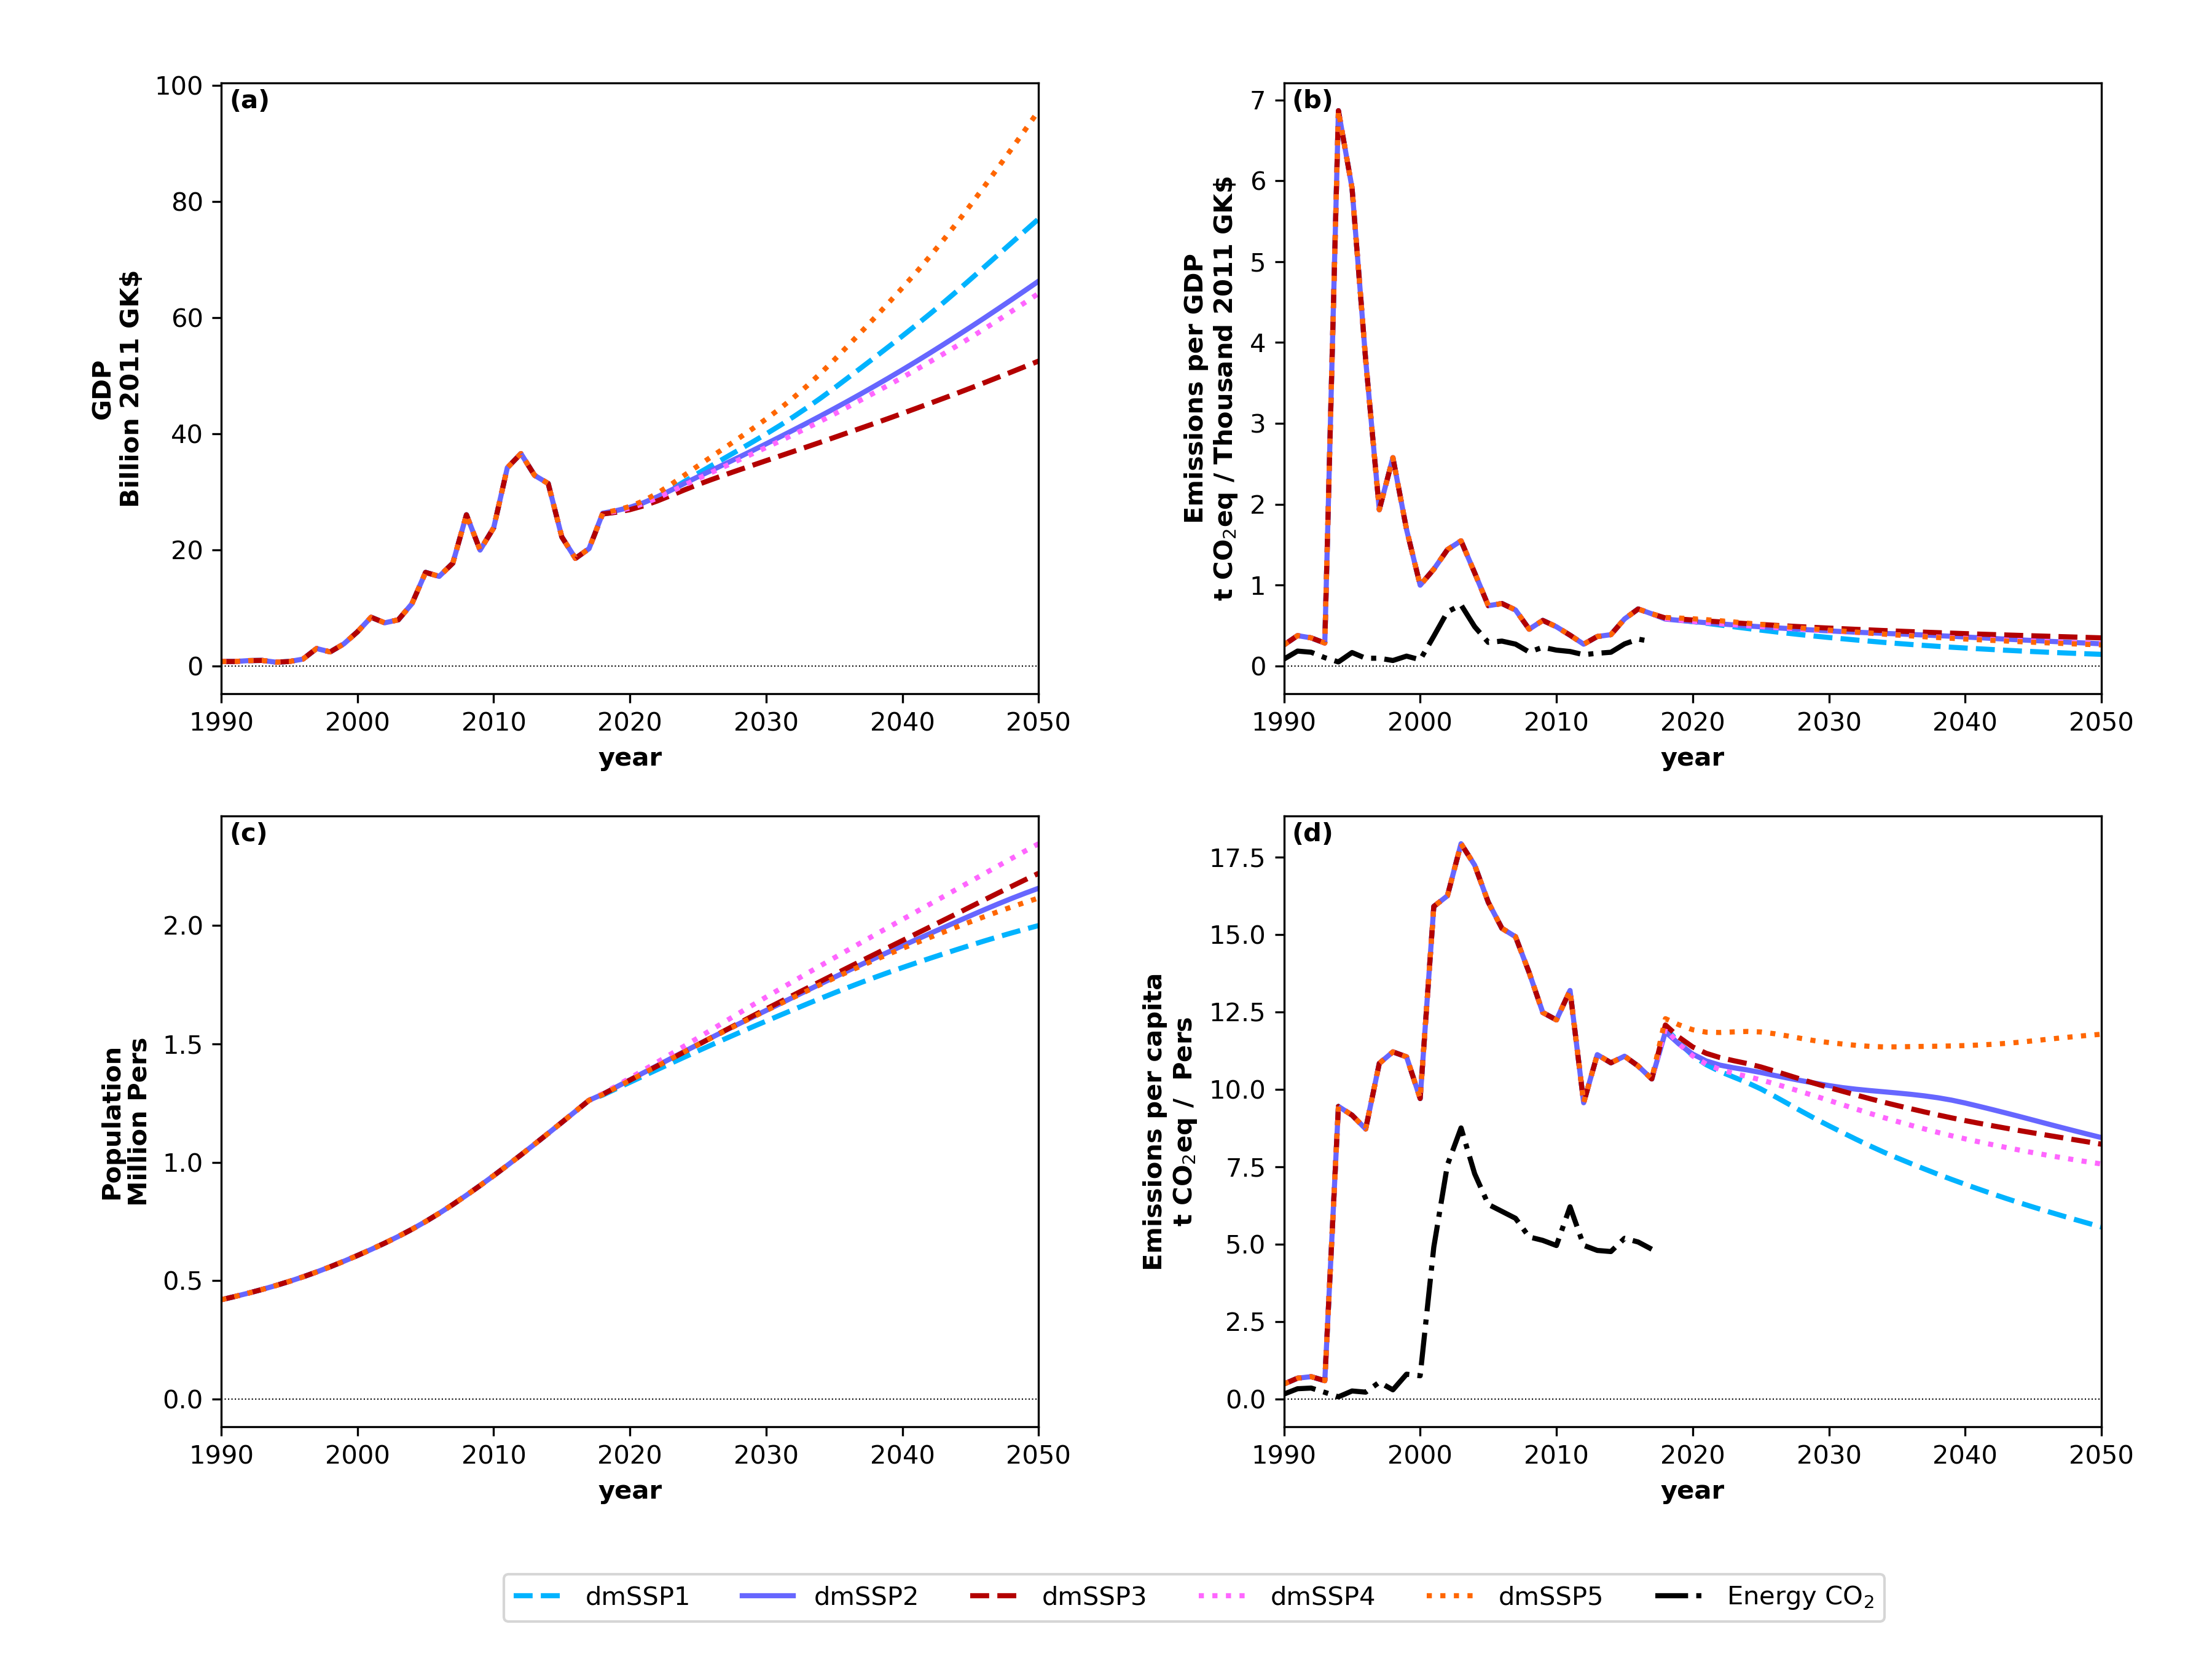
\includegraphics[width=\textwidth]{C:/Users/annikag/primap/ndc_quantifications/latex_files/GNQ/ts_gdp_pop_GNQ.png}
 \caption{Timeseries of national GDP (a) and population (c), and Kyoto~GHG emissions (exclLU, exclBunkers) per unit of GDP (b) or per capita (d).}
 \label{fig:tsSocioEco}
 \end{figure}

 The national GDP decreased in recent years, and the emissions per unit of GDP had a similar trend (Fig.~\ref{fig:tsSocioEco}).
 The population increased, while the per capita emissions were on the rise. 
 Following dmSSP2, the GDP is projected to increase towards 2050. 
 The emissions per GDP are estimated to decrease towars 2050. 
 Eq. Guinea's population is assumed to grow towards 2050, and the per capita emissions are expected to increase after 2017 but to decline again before 2050. 

 LULUCF emissions data for Eq. Guinea are available from the following sources (Fig.~\ref{fig:tsLULUCF}): FAO (2019)~/ 28, with the number of available data points in 1990--2017 displayed additionally.
 Based on data from FAO (2019), for the year 2017, LULUCF is estimated to be a net source of 5.4~Mt CO$_2$eq, which in absolute terms is lower than the non-LULUCF emissions of 13.0~Mt CO$_2$eq.
 The emissions range for FAO (2019) and 1990--2017 is 5.3--5.4~Mt CO$_2$eq.

 \begin{figure}[H]
 \centering
 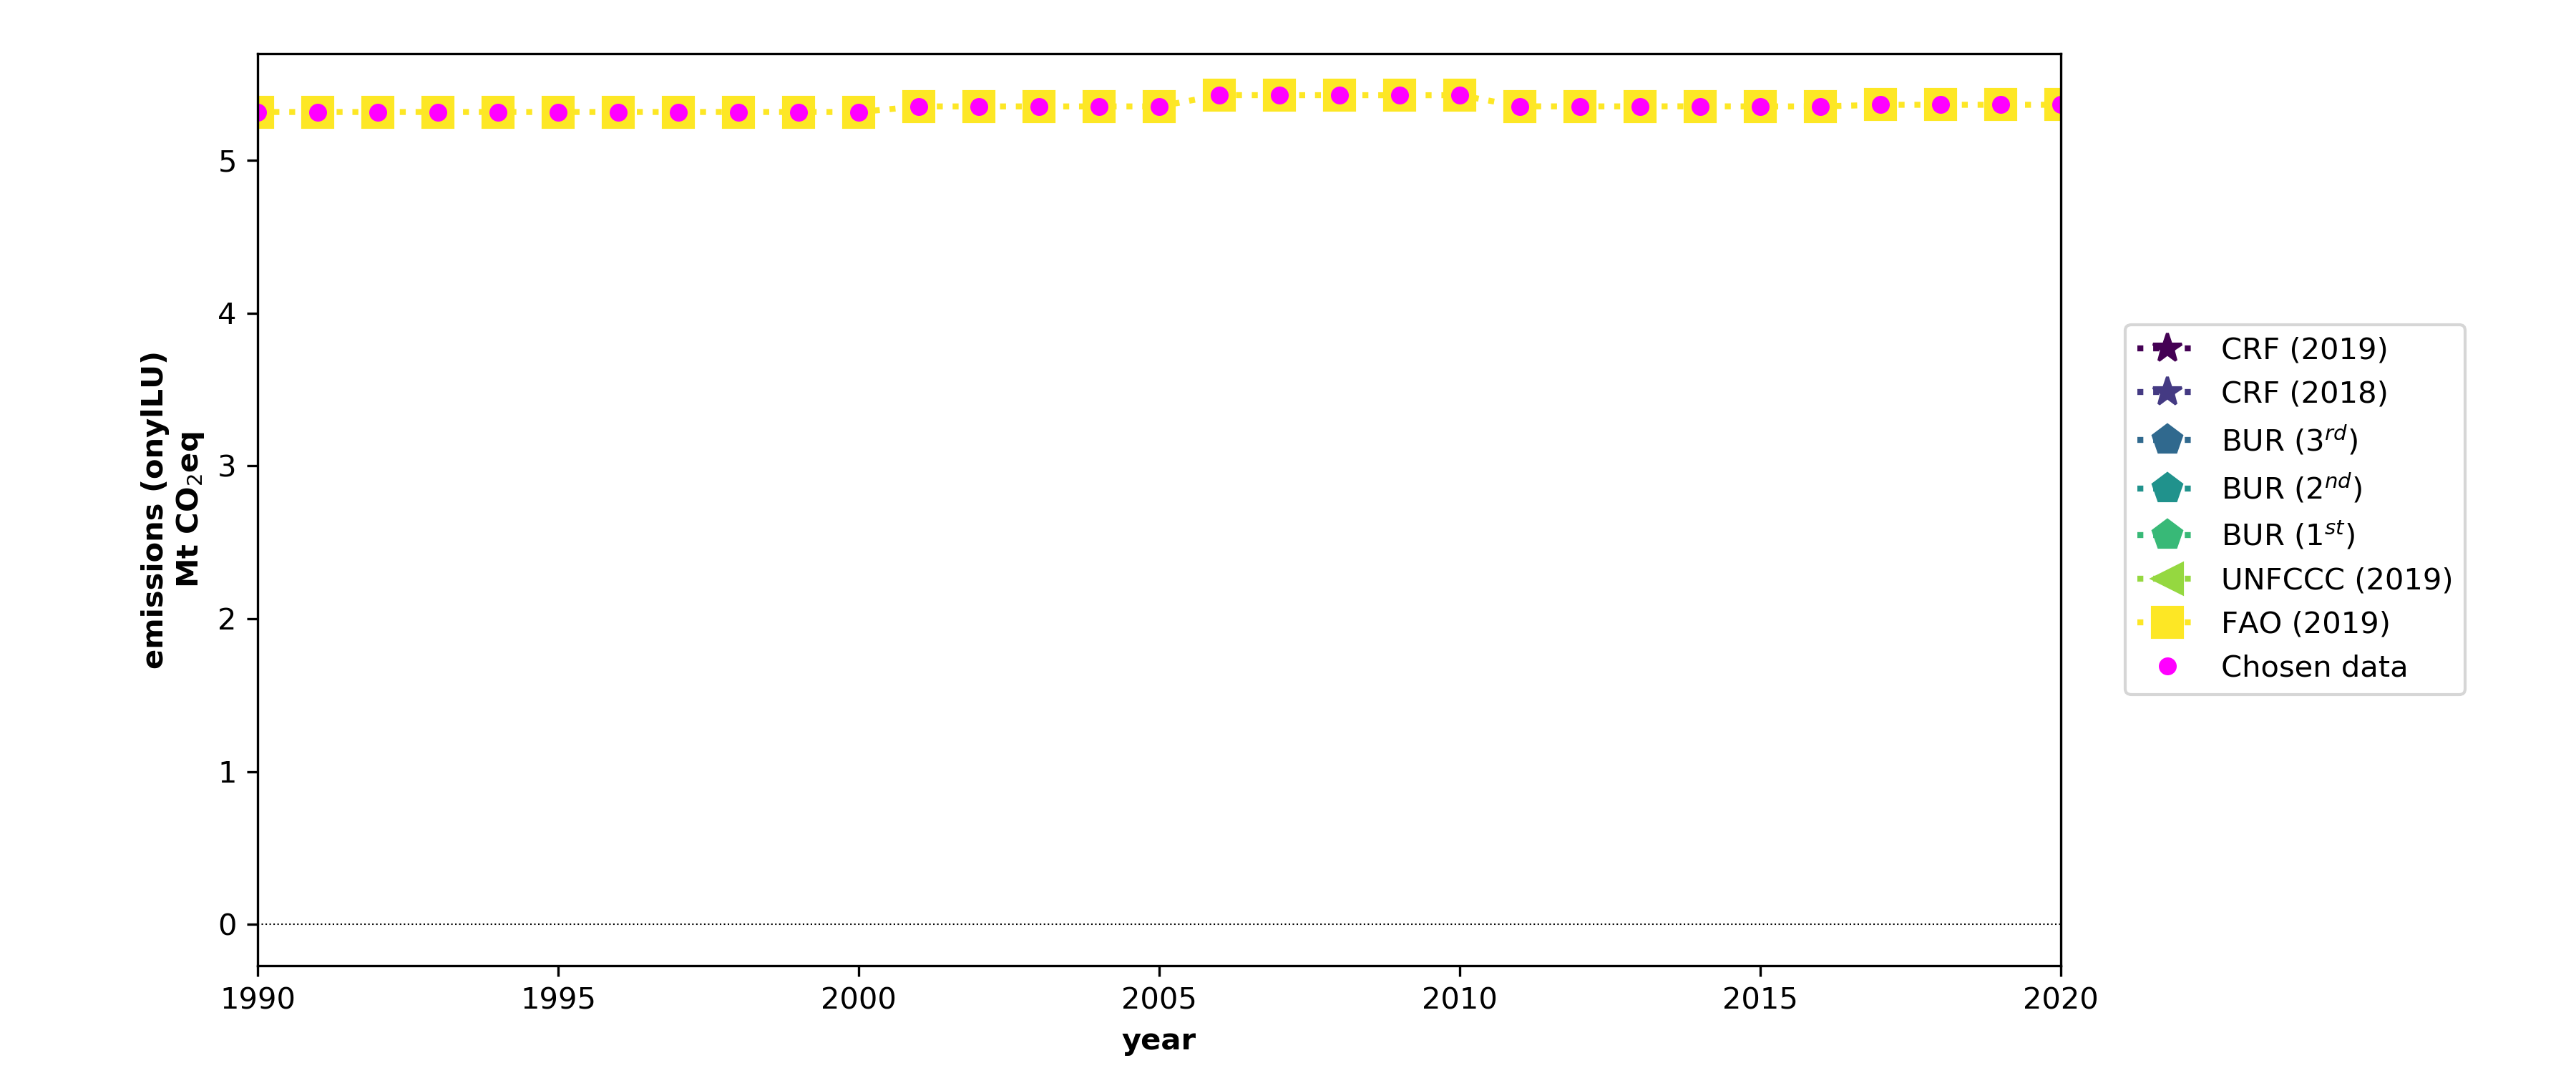
\includegraphics[width=\textwidth]{C:/Users/annikag/primap/ndc_quantifications/latex_files/GNQ/ts_emi_onlyLU_GNQ.png}
 \caption{Timeseries of emissions from LULUCF (CO$_2$ plus CH$_4$ and N$_2$O) as available from different data-sources. 
 Indicated in pink are the 'chosen' data, as used in our assessment of Eq. Guinea's NDC (if needed). 
 The pink timeseries was inter- and~/ or extrapolated (interpolation: linear, extrapolation: constant).}
 \label{fig:tsLULUCF}
 \end{figure}

 \newpage %%%
 \section{Mitigation targets (NDC)}
 \label{sec:mitiTars}

 \textbf{ 
 Give the \%cov for the base and target year (and 2017). \newline
 Global share for 2030 for the mitigated pathways and \% reduction relative to 1990 and 2017. \newline
 Table with the 'input' data and the resulting targets (like ndcs\_targets.csv). \newline}
 Eq. Guinea has an NDC, with a GHG mitigation target of the type RBY (base year target; main target type).
 The reclassified target type equals the main target type.

 \begin{table}[H]
 \centering
 \caption{Information on Eq. Guinea's GHG mitigation target(s).}
 \label{tab:mitiTars}
 \begin{tabular}{l l l l l l l }
 \bfseries type & \bfseries condi. & \bfseries range & \bfseries value & \bfseries refYr & \bfseries tarYr & \bfseries LU \tabularnewline \hline \hline
 RBY & condi. & best & -20\% & 2010 & 2030 & inclLU \tabularnewline 
 RBY & condi. & best & -50\% & 2010 & 2050 & inclLU \tabularnewline 
 \end{tabular}
 \end{table}

 \begin{figure}[H]
 \centering
 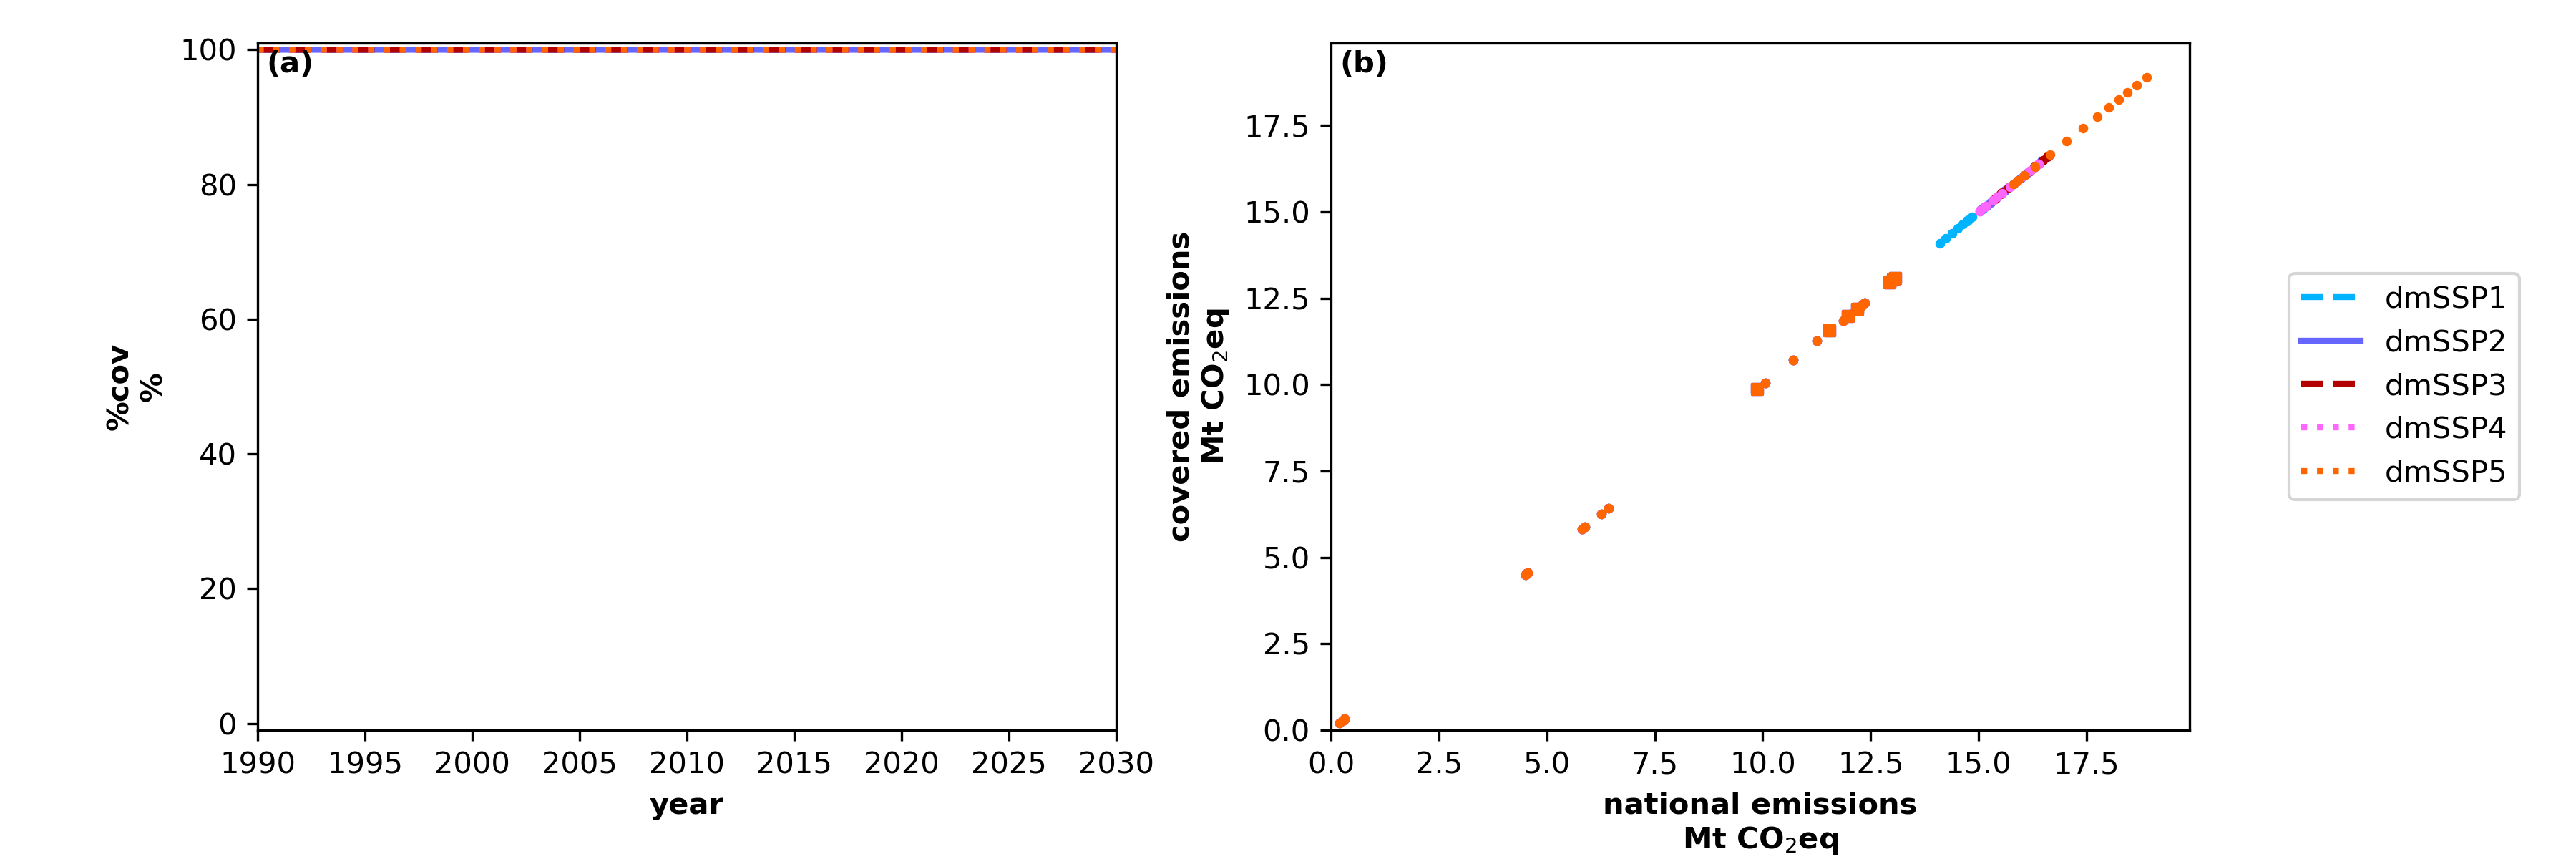
\includegraphics[width=\textwidth]{C:/Users/annikag/primap/ndc_quantifications/latex_files/GNQ/ts_pc_cov_GNQ.png}
 \caption{Timeseries of Eq. Guinea's national emissions (exclLU) and the share of emissions that is assumed to be covered by Eq. Guinea's mitigation target.}
 \label{fig:tsPcCov}
 \end{figure}

 \begin{table}[H]\small
 \centering
 \caption{Information on covered sectors and gases as retrieved from NDC and adapted ('Adap.': used to calculate \%cov), and their shares in Eq. Guinea's 2017 emissions (exclLU, exclBunkers; total 13.0~Mt CO$_2$eq).
 If either the sector or gas is assessed as 'not-covered', the emissions from this sector-gas combination are counted as not-covered (--). 
 Else the emissions are counted as covered (+; covered shares given in bold).
 (/) means that no information is available.
 LULUCF: NDC '+' and adapted '+' (estimated as a net source of 5.4~Mt CO$_2$eq in 2017; based on the 'chosen' LULUCF emissions).}
 \label{tab:coveredSectorsGases}
 \begin{tabular}{l || c c || c c c c c c c | c}
 \bfseries  & \bfseries NDCs & \bfseries Adap. & \bfseries CO$_2$ & \bfseries CH$_4$ & \bfseries N$_2$O & \bfseries HFCs & \bfseries PFCs & \bfseries SF$_6$ & \bfseries NF$_3$ & \bfseries Total \tabularnewline \hline \hline
 \bfseries NDCs &  &  & / & / & / & / & / & / & / &  \tabularnewline 
 \bfseries Adap. &  &  & \bfseries + & \bfseries + & \bfseries + & -- & -- & -- & -- &  \tabularnewline \hline \hline
 \bfseries Energy & \bfseries + & \bfseries + & \bfseries 46.8\% & \bfseries 40.9\% & \bfseries 0.1\% & / & / & / & / & 87.8\% \tabularnewline 
 \bfseries IPPU & \bfseries + & \bfseries + & \bfseries 8.6\% & \bfseries 0.7\% & \bfseries 0.0\% & / & / & / & / & 9.3\% \tabularnewline 
 \bfseries Agri. & \bfseries + & \bfseries + & \bfseries / & \bfseries 0.1\% & \bfseries 0.07\% & / & / & / & / & 0.1\% \tabularnewline 
 \bfseries Waste & \bfseries + & \bfseries + & \bfseries / & \bfseries 2.7\% & \bfseries 0.0\% & / & / & / & / & 2.7\% \tabularnewline 
 \bfseries Other & / & \bfseries + & \bfseries / & \bfseries / & \bfseries 0.03\% & / & / & / & / & 0.03\% \tabularnewline \hline
 \bfseries Total &  &  & 55.4\% & 44.3\% & 0.2\% & / & / & / & / & 100.0\% \tabularnewline 
 \end{tabular}
 \end{table}

 \begin{figure}[H]
 \centering
 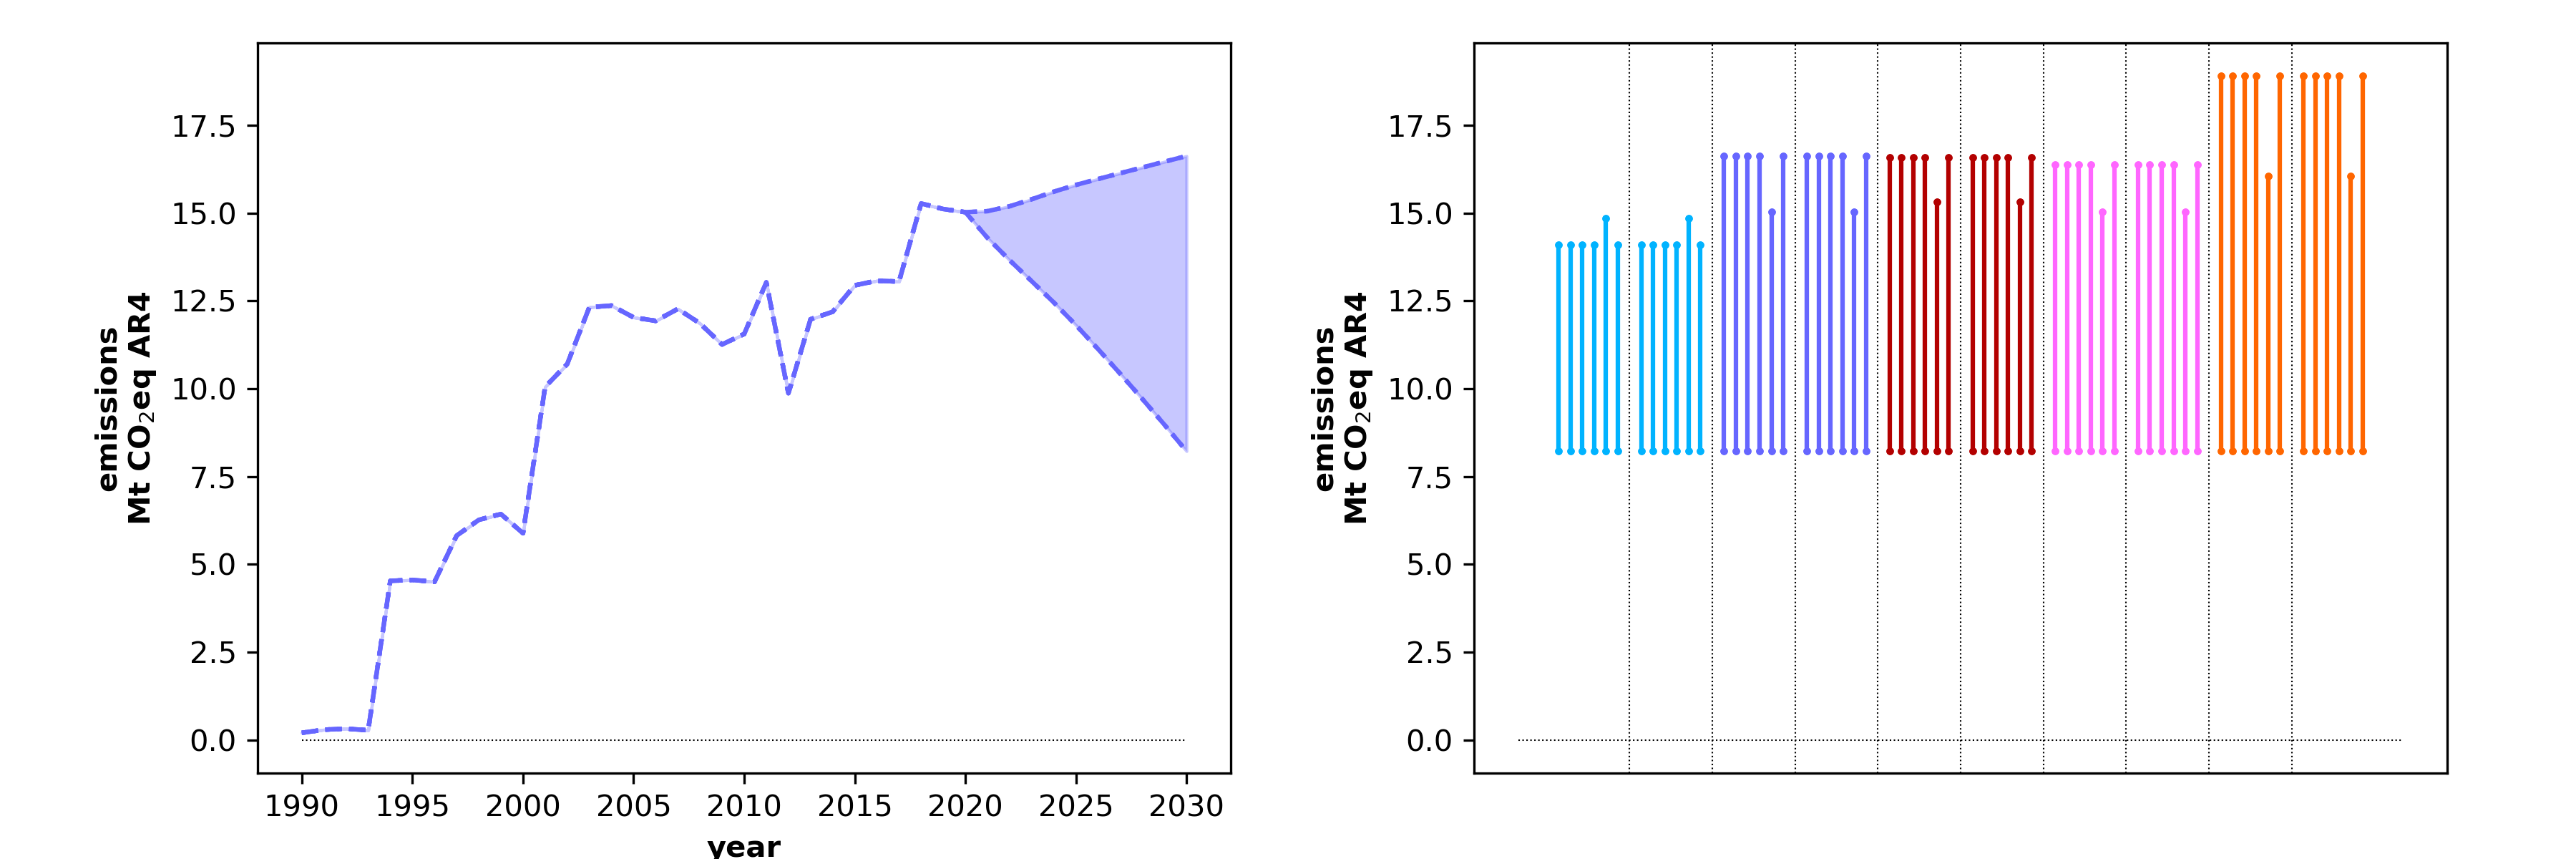
\includegraphics[width=\textwidth]{C:/Users/annikag/primap/ndc_quantifications/latex_files/GNQ/ts_ndcs_quantis_GNQ.png}
 \caption{Quantified mitigation targets (based on different input data and calculation options).
 Vertical lines: conditionality~/ range;
 colour coded: dmSSP1--5;
 first~/ second set of six: prio NDCs~/ SSPs;
 set of six: coverage 100, lulucf unfccc, lulucf fao, bl uncondi, const emi, estimated coverage.}
 \label{fig:miti}
 \end{figure}

 \newpage %%%
 \section{Data sources, additional information and references}
 \label{sec:dataSourcesRefs}

 \noindent \href{https://dataservices.gfz-potsdam.de/pik/showshort.php?id=escidoc:4736895}{PRIMAP-hist v2.1}: emissions from PRIMAP-hist are data from the country reported data priority scenario (HISTCR).

 \noindent \href{https://zenodo.org/record/3638137#.X2syXouxU2w}{dmSSPs}: emissions, population and GDP data are PMSSPBIE data for the five marker scenarios.

 \begin{description}
 \item [SSPs] Shared Socio-economic Pathways. \newline
 Narratives and challenges to mitigation and adaptation: \newline
 \textit{SSP1}: Sustainability, Taking the Green Road (low~/ low); \newline
 \textit{SSP2}: Middle of the Road (medium~/ medium); \newline
 \textit{SSP3}: Regional Rivalry, A Rocky Road (high~/ high); \newline
 \textit{SSP4}: Inequality, A Road Divided (low~/ high); and \newline
 \textit{SSP5}: Fossil-fuelled Development, Taking the Highway (high~/ low).
 \item [GDP] Gross Domestic Product. \newline
 Throughout this document the GDP is given as GDP~PPP, with PPP being the Purchasing Power Parity.
 \item [GWP] Global Warming Potential. \newline
 We use GWP values from the IPCC 4$^{th}$ Assessment Report (AR4). 
 They reflect the forcing potential of one kilogram of a gas' emissions in comparison to one kilogram of CO$_2$ (GWP$_{CO2}$ = 1). 
 The GWPs correspond to a 100-yr period and are for CH$_4$:~25, for N$_2$O:~298, for SF$_6$:~22800, and for NF$_3$:~17200. 
 For the basket of HFC-gases the GWPs from AR4 are in the range 4--14800, and for PFCs 7190--12200. 
 To assess emissions of several GHGs, their emissions are weighted by their respective GWPs and presented in CO$_2$ equivalents (CO$_2$eq).
 \item [LULUCF] Land Use, Land-Use Change and Forestry. \newline
 Emissions from LULUCF are excluded throughout the document, unless stated otherwise.
 \item [Bunkers fuels] Emissions from international aviation and shipping.
 \item [Kyoto~GHG] Kyoto~GHG (Greenhouse Gas) basket. \newline
 Carbon dioxide (CO$_2$), methane (CH$_4$), nitrous oxide (N$_2$O), hydrofluorocarbons (HFCs), perfluorocarbons (PFCs), sulfur hexafluoride (SF$_6$), and nitrogen trifluoride (NF$_3$).
 \item [F-gases] Fluorinated gases. \newline
 Basket of HFCs, PFCs, and the gases SF$_6$ and NF$_3$. 
 Some F-gases have very long atmospheric lifetimes and high Global Warming Potentials.
 \item [Target reclassification] When a country has, e.g., an RBU target (relative reduction compared to Business-As-Usual), and the BAU emissions are provided, it can be quantified based on the given emissions, and is reclassified from type\_main~RBU to type\_reclass~ABS (absolute emissions target).
 Additionally, 'NGT' targets can be reclassified as 'ABU' (absolute reduction compared to Business-As-Usual) if absolute mitigation effects due to planned policies and measures are provided.
 \item [Quantification options] Different quantification options were tested. \newline
 \textit{dmSSP1--5}: down-scaled SSP marker scenarios; \newline
 \textit{type\_reclass}: external data prioritised (PRIMAP-hist, dmSSPs); \newline
 \textit{type\_main}: emissions data from within NDCs were prioritised; \newline
 \textit{100\% coverage \& estimated coverage}; \newline
 \textit{constant~emi}: constant emissions after last target year (instead of constant relative difference to baseline); \newline
 \textit{baseline uncondi}: baseline emissions as uncond. pathways for Parties without uncond. targets, even if baseline is better than cond. targets (instead of cond. pathway as uncond. pathways in these cases).
 \end{description}

 \noindent \textbf{Links to additional information:}
 \begin{itemize}
 \item \href{https://www.climatewatchdata.org/}{CLIMATEWATCH} 
 \vspace{-.2cm} \item \href{https://www.carbonbrief.org/}{CarbonBrief: Clear on Climate} 
 \vspace{-.2cm} \item \href{https://uk.reuters.com/article/us-climate-change-china/chinas-carbon-neutral-pledge-could-curb-global-warming-by-0-3c-researchers-idUKKCN26E325?utm_campaign=Carbon%20Brief%20Daily%20Briefing&utm_medium=email&utm_source=Revue%20newsletter}{China's carbon neutral pledge could curb global warming by 0.3$^{\circ}$C~- researchers} (23 September 2020)
 \vspace{-.2cm} \item \href{https://climateactiontracker.org/}{Climate Action Tracker} 
 \vspace{-.2cm} \item \href{https://www.bbc.com/news/science-environment-54274644?utm_campaign=Carbon%20Brief%20Daily%20Briefing&utm_medium=email&utm_source=Revue%20newsletter}{Coronavirus: Climate action cannot be another Covid victim~- PM} (23 September 2020)
 \vspace{-.2cm} \item \href{https://www.wri.org/blog/2019/07/countries-climate-plans-ndcs-are-missing-big-opportunity-reducing-food-loss-and-waste}{Countries' Climate Plans (NDCs) Are Missing a Big Opportunity: Reducing Food Loss and Waste} (3 July 2019)
 \vspace{-.2cm} \item \href{https://zenodo.org/record/3638137#.X2sqPIuxU2w}{Country resolved combined emission and socio-economic pathways based on the RCP and SSP scenarios} (February 2020)
 \vspace{-.2cm} \item \href{https://www.theguardian.com/environment/2020/sep/23/few-countries-living-up-to-green-recovery-promises-analysis?utm_campaign=Carbon%20Brief%20Daily%20Briefing&utm_medium=email&utm_source=Revue%20newsletter}{Few countries living up to Covid 'green recovery' pledges~- analysis} (23 September 2020)
 \vspace{-.2cm} \item \href{https://www.carbonbrief.org/guest-post-calculating-the-true-climate-impact-of-aviation-emissions?utm_campaign=Carbon%20Brief%20Daily%20Briefing&utm_medium=email&utm_source=Revue%20newsletter}{Guest post: Calculating the true climate impact of aviation emissions} (September 2020)
 \vspace{-.2cm} \item \href{https://www.iges.or.jp/en/pub/iges-indc-ndc-database/en}{IGES NDC Database} 
 \vspace{-.2cm} \item \href{https://www.ipcc.ch/}{IPCC (The Intergovernmental Panel on Climate Change)} 
 \vspace{-.2cm} \item \href{https://www.ipcc.ch/sr15/}{IPCC Special Report: Global Warming of 1.5$^{\circ}$} (2018)
 \vspace{-.2cm} \item \href{https://www.isimip.org/isipedia/#isipedia-portal}{ISIMIP~/ ISIpedia} 
 \vspace{-.2cm} \item \href{https://www.theguardian.com/environment/2020/sep/23/melting-antarctic-ice-will-raise-sea-level-by-25-metres-even-if-paris-climate-goals-are-met-study-finds?CMP=share_btn_tw&utm_campaign=Carbon%20Brief%20Daily%20Briefing&utm_medium=email&utm_source=Revue%20newsletter}{Melting Antarctic ice will raise sea level by 2.5 metres~- even if Paris climate goals are met, study finds} (23 September 2020)
 \vspace{-.2cm} \item \href{https://klimalog.die-gdi.de/ndc/#NDCExplorer/worldMap?NDC??income???catIncome}{NDC Explorer} 
 \vspace{-.2cm} \item \href{https://ndcpartnership.org/}{NDC PARTNERSHIP} 
 \vspace{-.2cm} \item \href{https://themasites.pbl.nl/o/climate-ndc-policies-tool/}{PBL Climate Pledge NDC tool} 
 \vspace{-.2cm} \item \href{https://tntcat.iiasa.ac.at/SspDb/dsd?Action=htmlpage&page=about}{SSP Database (Shared Socioeconomic Pathways)~- Version 2.0} (December 2018)
 \vspace{-.2cm} \item \href{https://dataservices.gfz-potsdam.de/pik/showshort.php?id=escidoc:4736895}{The PRIMAP-hist national historical emissions time series (1850-2017)} (2019)
 \vspace{-.2cm} \item \href{https://unfccc.int/}{UNFCCC (United Nations Framework Convention on Climate Change)} 
 \vspace{-.2cm} \item \href{https://www.wri.org/}{WORLD RESOURCES INSTITUTE} 
 \vspace{-.2cm} \item \href{https://www.washingtonpost.com/weather/2020/09/23/atlantic-hurricanes-record-2020/?utm_campaign=Carbon%20Brief%20Daily%20Briefing&utm_medium=email&utm_source=Revue%20newsletter}{Why the 2020 Atlantic hurricane season has spun out of control: Extra-warm ocean waters, boosted by climate change, and La Ni{\~n}a are key drivers in historic season.} (September 2020)
 \vspace{-.2cm} \item \href{https://www.theguardian.com/environment/2020/sep/21/worlds-richest-1-cause-double-co2-emissions-of-poorest-50-says-oxfam?utm_campaign=Carbon%20Brief%20Daily%20Briefing&utm_medium=email&utm_source=Revue%20newsletter}{World's richest 1\% cause double CO$_2$ emissions of poorest 50\%, says Oxfam} 
 \vspace{-.2cm} \item \href{https://www.showyourbudgets.org/de/?country=whole_world}{\#showyourbudgets} 
 \end{itemize}

 %%%
 \end{document}
